\chapter{Conclusiones y trabajo futuro}

Las aproximaciones de la distribución posterior dadas por las aproximaciones del forward map son en general útiles y simples de manejar. En cada uno de los tres modelos estudiados se llegó a que existe una aproximación decente con un menor tiempo de ejecución. Sin embargo, aunque es cierto que comparaciones uno a uno el método aproximado es mejor en tiempo de ejecución, no lo es en conjunto. Esto quiere decir, que la investigación de la mejor aproximación conlleva una mayor inversión temporal. 
Más aún, considérese que la experimentación se ha realizado con aproximaciones del forward map de la misma cantidad de vecinos cercanos y misma resolución de malla teniendo un grado de aproximación óptimo con tres vecinos y una definición de malla de 50  en cada uno de los modelos presentados. Por razonamiento inductivo, podemos conjeturar que tendremos una aproximación decente en cualquier otro modelo de EDO's con la misma regla de aproximación, esperando una mejora en el tiempo de ejecución previo a realizar la metodología con forward map ordinario. 

Cabe resaltar que las aproximaciones hechas con más vecinos fueron rechazadas por deficiencia de la convergencia experimental en la distribución posterior. Este caso se atribuye a que agregar muchos vecinos, como lo fue para aproximaciones de $8$ vecinos cercanos, añade a la aproximación de la distribución posterior un \textit{ruido} que perturba considerablemente la distribución posterior resultante.

Por otro lado, la incorporación de la regulación de las unidades tomó un papel fundamental para la metodología aproximada. En teoría hemos visto que la ausencia de esta resulta en aproximaciones sesgadas a aquellos parámetros cuyas unidades sean la de menor orden de magnitud. En la práctica, el uso de la metodología sin la regularización de las unidades produce aproximaciones burdas para los parámetros con mayor orden de magnitud. En el caso del modelo SIR, considerar la resolución del problema inverso sin la regularización de las unidades, ocasiona que la distribución posterior aproximada, solo aproxima marginalmente para $\beta$. Esto se debe a que sin la regularización de las unidades y debido a la construcción ponderada  inversamente a la distancia en el forward map aproximado, es que el orden de magnitud de las unidades de $\gamma$ al ser mayores que las mismas de $\beta$, son insignificantes para la aproximación ocasionando el sesgo mencionado. Veamos el caso de cinco vecinos cercanos en la Fig. \ref{Fig. Regulacion_1}
y el caso de ocho vecinos cercanos en la Fig. \ref{Fig. Regulacion_2} sin la regularización de las unidades.

\begin{figure}[H] 
    \centering 
    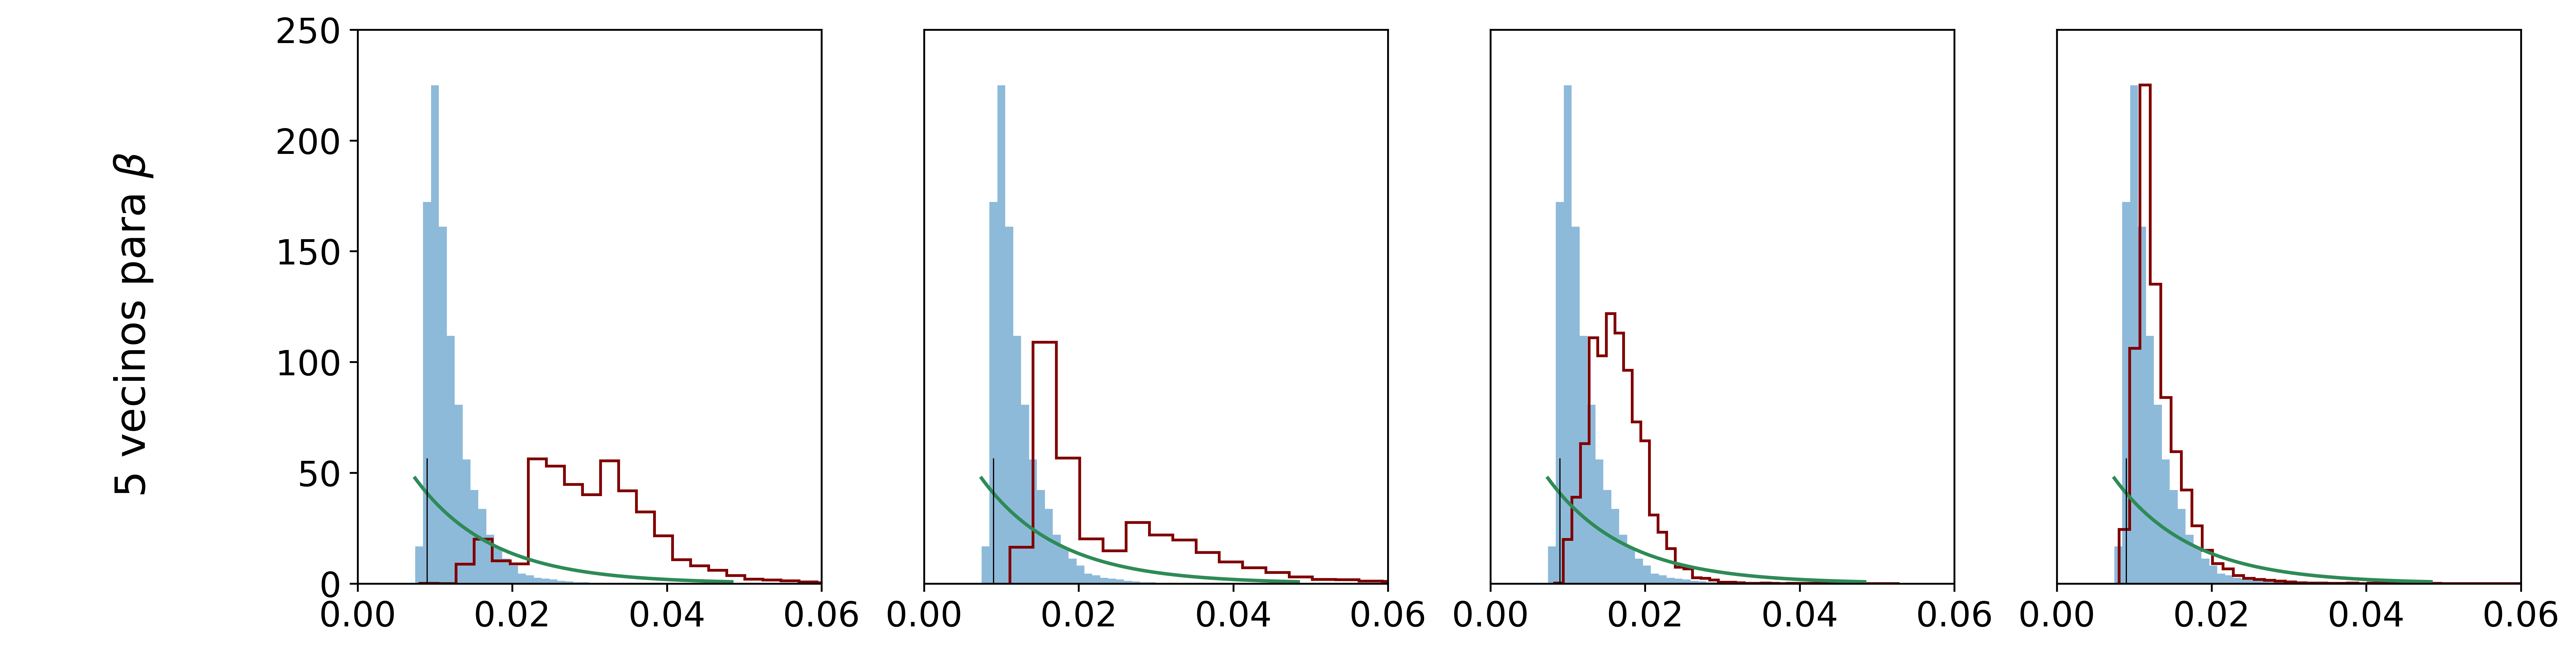
\includegraphics[width = 17 cm ]{img/Unidades_1.png} 
    % \caption{}
    % \label{Fig. }
\end{figure} 
\begin{figure}[H] 
    \centering 
    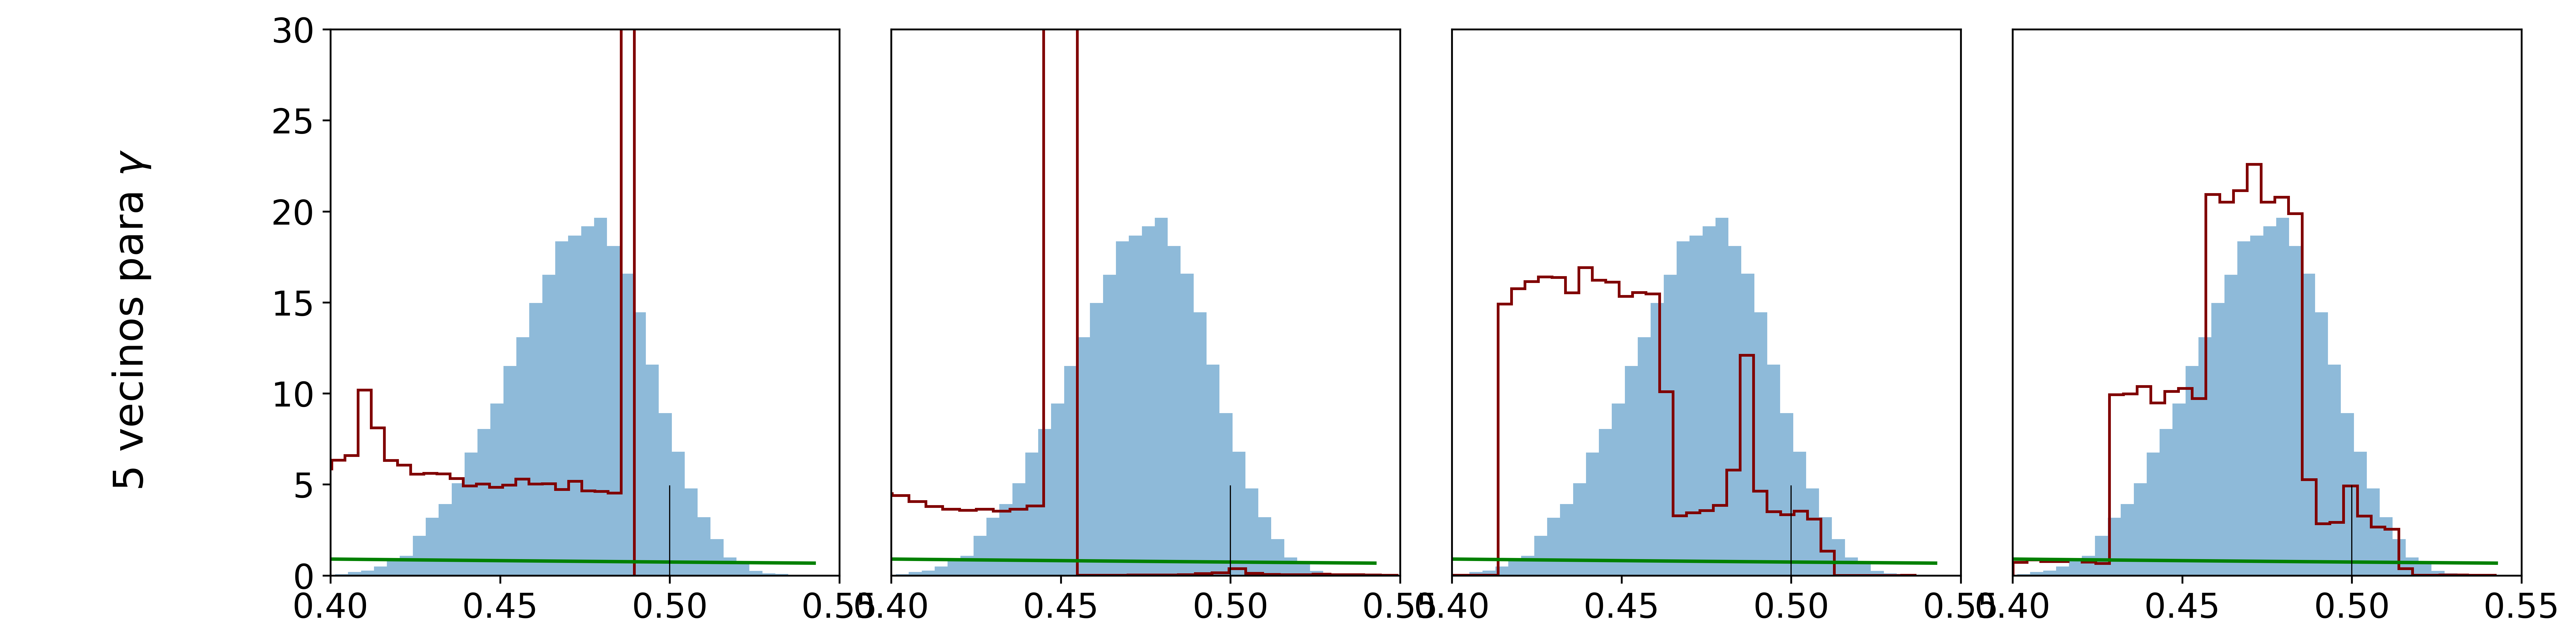
\includegraphics[width = 17 cm ]{img/Unidades_2} 
    \caption{Distribuciones marginales posteriores aproximadas (rojo) con forward map aproximado a cinco vecinos cercanos y una malla de resolución 10,15,30,50 de izquierda a derecha, sin regularización de las unidades. En azul la distribución posterior con forward map ordinario para modelo SIR.}
    \label{Fig. Regulacion_1}
\end{figure} 

\begin{figure}[H] 
    \centering 
    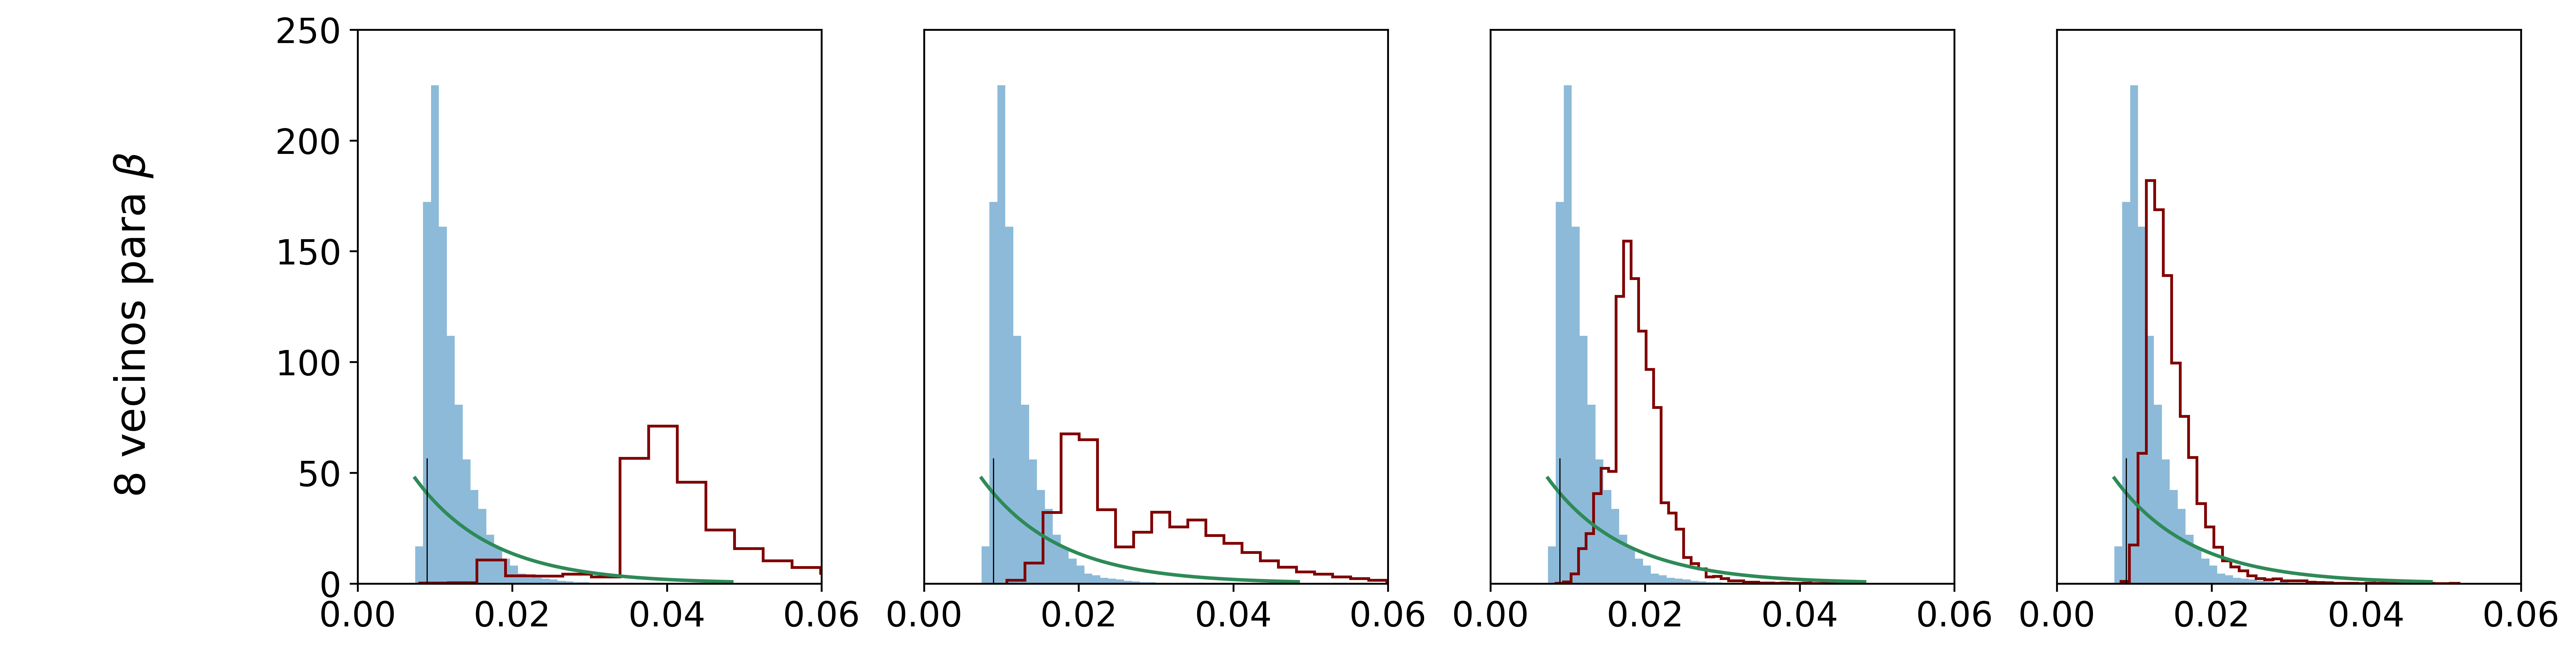
\includegraphics[width = 17 cm ]{img/Unidades_3.png} 
    % \caption{}
    % \label{Fig. }
\end{figure} 
\begin{figure}[H] 
    \centering 
    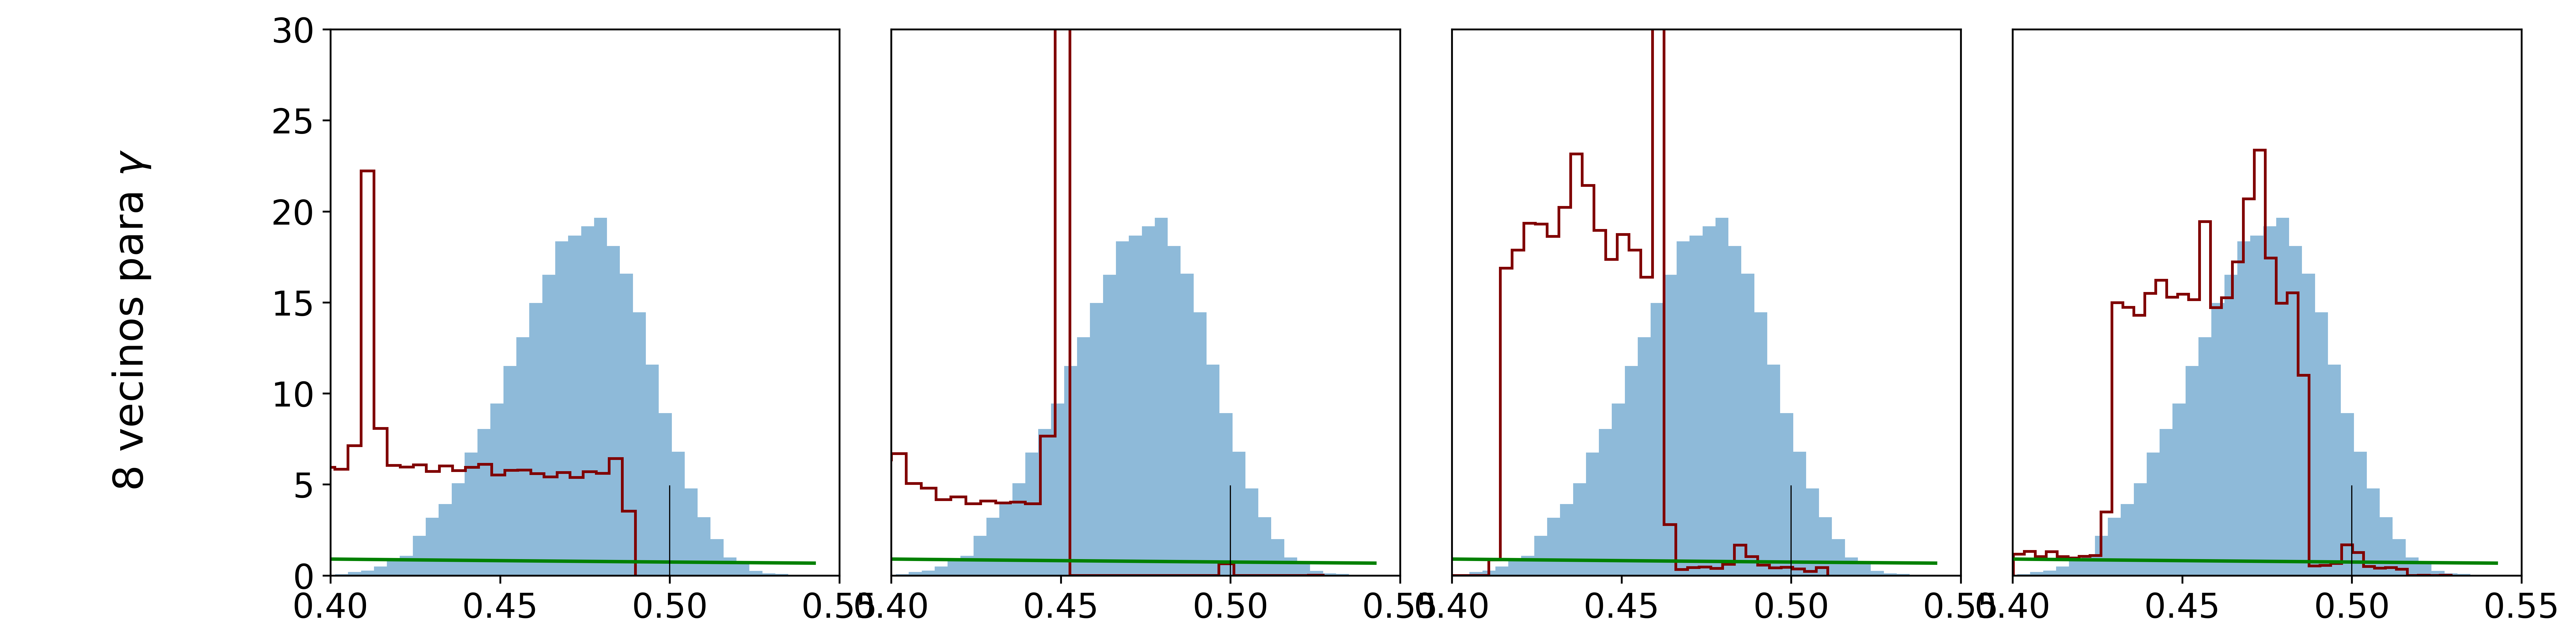
\includegraphics[width = 17 cm ]{img/Unidades_4} 
    \caption{Distribuciones marginales posteriores aproximadas (rojo) con forward map aproximado a ocho vecinos cercanos y una malla de resolución 10,15,30,50 de izquierda a derecha, sin regularización de las unidades. En azul la distribución posterior con forward map ordinario para modelo SIR.}
    \label{Fig. Regulacion_2}
\end{figure} 

Existen multiples formas de mejorar el algoritmo para la solución del problema inverso en modelos dados por EDO's. Una de ellas considerada a trabajo futuro es la creación de mallas no rectangulares, que además se vaya construyendo de forma adaptativa, esto quiere decir que se deje correr la cadena del algoritmo Metropolis-Hastings de forma ordinaria una cantidad fija de iteraciones y en cada paso se construya la malla. Esto con la idea de que los puntos de la discretización que son poco probables no se vean sobre-representados.

También considerado a futuro, es de interés trabajar con distintos modelos de EDO's a los presentados en este proyecto, pues de esta forma se podrían encontrar casos en los que la metodología aproximada propuesta aquí resulte con irregularidades, donde el tratamiento de estas conlleve a la mejora del algoritmo. Además de irregularidades como la que sucede en el modelo logístico, vea la Fig. \ref{Fig. Aprox log 3v}, donde se muestra un sesgo a la izquierda de la distribución posterior aproximada pese a que ya se regularizaron las unidades.

Por otro lado, es de interés implementar cuantitativamente el grado de aproximación que tiene las posteriores con su análogo ordinario. Proponiendo la implementación de las distancias de Kullback-Leibler como sustitución de la simple inspección de la aproximación.